\scanpage{51}
$A=(\underline Z/n\underline Z)_Y$ comme simple corollaire, mais ça m'étonnerait. La même remarque s'applique d'ailleurs également au théorème de dualité globale, qui s'énonce pour des faisceaux d'anneaux plus généraux que le faisceau constant $\underline Z/n\underline Z$.
\figure{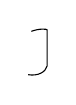
\begin{tikzpicture}[x=0.1cm,y=0.1cm]\draw(0,5.5)..controls(1,5.9)and(2,5.8)..(2,5.7)--(2,1.1)..controls(1.8,0.3)and(0.8,-0.2)..(-0.4,0);\end{tikzpicture}}

Il me semble que la relation de nature transcendante qui lie la cohomologie de De-Rham ou de Hodge aux cohomologies $\ell$-adiques, lorsque le corps de base est $\underline C$, via la cohomologie entière, devrait avoir un\deleted{\unsure{e relati|relati}}\deleted{\unsure{on|en}} analogue lorsque le corps de base est \inserted{alg clos} valué complet non archimédien, à corps résiduel de caractéristique p, \deleted{\unsure{caractéristique}} et corps des fractions \inserted{K} de caractéristique zéro,savoir que $H^*(X,\underline Z_p)$ doit s'envoyer alors de façon $\underline Z_p$-linéaire dans la cohomologie de De\unsure{-}Rham $H^*(X)$, qui serait isomorphe alors à $H^*(X,\underline Z_p)\otimes_{\underline Z_p}K$. Pour définir un tel homomorphisme, on pourrait penser à utiliser l'espace rigide-analytique au sens de Tate défini par X (NB c'est un site qui ne peut être défini par une topologie au sens ordinaire, ce qui explique les difficultés conceptuelles initiales de Tate pour arriver à définir la notion d'espace rigide-analytique), soit $X^{\mathrm{an}}$. On espère que les arguments habituels prouveront que pour des fais\deleted{\unsure{ce}}ceaux de torsion, la cohomologie de $X_{\text{ét}}$ coïncide avec celle de $X^{\mathrm{an}}$, et un excès d'optimisme nous ferait espérer que la cohomologie de $X^{\mathrm{an}}$ à coéfficients constants $\underline Z_p$ est bien la limite projective des cohomologies à coéfficients dans les $\underline Z/p^n\underline Z$, donc coïncide avec la cohomologie p-adique $H(X_{\text{ét}},\underline Z_p)$ (définie précisément comme une limite analogue). Si cela était vrai, l'immersion canonique de $\underline Z_p$ dans les fonctions constantes sur $X^{\mathrm{an}}$ semblerait permettre d'envoyer $H(X^{\mathrm{an}},\underline Z_p)$ dans la cohomologie de De Rham de $X^{\mathrm{an}}$, qui par Gaga rigide-analytique n'est autre que celle de X. L' ``excès'' plus haut serait justifié essentiellement par un ``lemme
\margin{50}
